% !TEX program = xelatex
\documentclass[11pt]{article}
\usepackage{fontspec}

\setsansfont{Palatino}[
    Path=./palatino/,
    Extension = .ttf,
    UprightFont=*-Roman,
    BoldFont=*-Bold,
    ItalicFont=*-Italic,
    BoldItalicFont=*-BoldItalic
]
\setmainfont{Palatino}

\usepackage[textwidth=0.86\paperwidth, textheight=0.86\paperheight]{geometry}
\usepackage{fancyhdr}
\usepackage{hyperref}
\usepackage{fontawesome5}
\usepackage{graphicx}
\usepackage{amssymb}
\usepackage{amsmath}

\newcommand{\R}{\mathbb{R}}

\begin{document}

% Set the page style to "fancy"...
\pagenumbering{gobble}
\pagestyle{fancy}
\fancyhead{} % clear all header fields
\fancyhead[R]{\href{https://mipt23.fmin.xyz}{\faGem[regular]} \hspace{0.04cm} \href{https://github.com/MerkulovDaniil/mipt23}{\faGithub} \hspace{0.07cm} \href{https://t.me/fminxyz}{\faTelegram}}
\fancyhead[L]{\href{https://fmin.xyz}{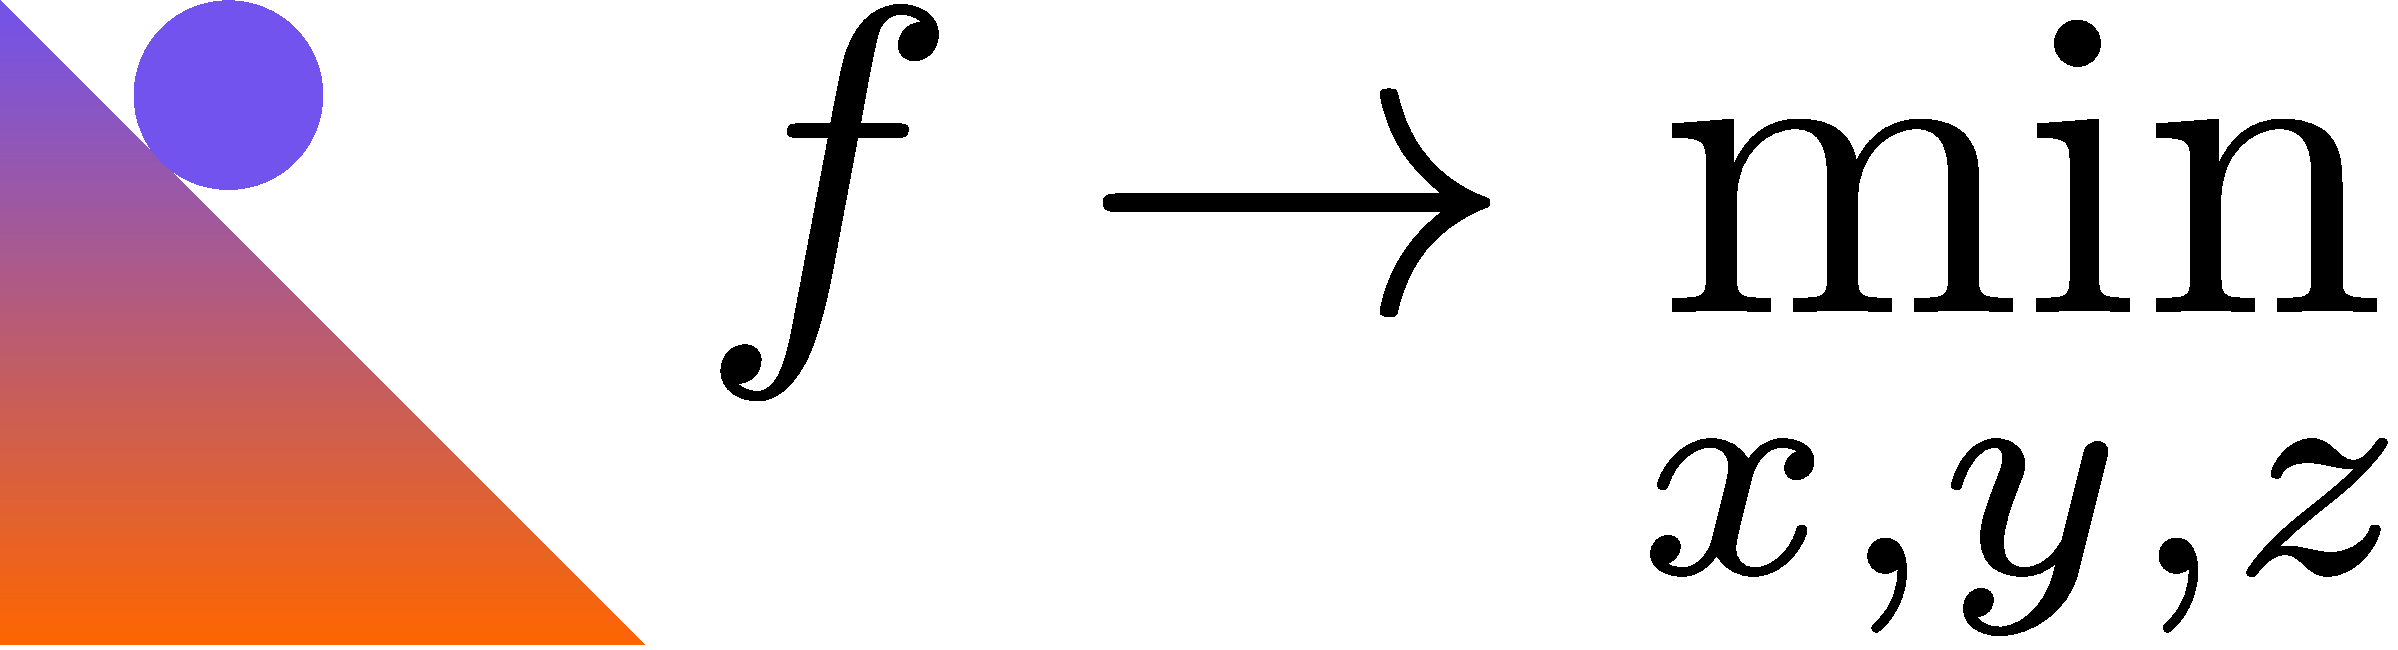
\includegraphics[height=0.35cm]{logo.pdf}} \hspace{2pt} \textbf{Методы оптимизации. МФТИ. Экзамен. Декабрь 2023}}



\section*{Определения и формулировки}
\begin{enumerate}
    \setlength\itemsep{-0.3em}
    \item Положительно определённая матрица.
    \item Евклидова норма вектора.
    \item Неравенство треугольника для нормы.
    \item $p$-норма вектора.
    \item Как выглядит единичный шар в $p$ - норме на плоскости для $p=1,2,\infty$?
    \item Норма Фробениуса для матрицы.
    \item Спектральная норма матрицы.
    \item Скалярное произведение двух векторов.
    \item Скалярное произведение двух матриц, согласованное с нормой Фробениуса.
    \item Собственные значения матрицы. Спектр матрицы.
    \item Связь спектра матрицы и её определенности.
    \item Спектральное разложение матрицы.
    \item Сингулярное разложение матрицы.
    \item Связь определителя и собственных чисел для квадратной матрицы.
    \item Связь следа и собственных чисел для квадратной матрицы.
    \item Градиент функции $f(x): \R^n \to \R$.
    \item Гессиан функции $f(x): \R^n \to \R$.
    \item Якобиан функции $f(x): \R^n \to \R^m$.
    \item Формула для аппроксимации Тейлора первого порядка $f^I_{x_0}(x)$ функции $f(x): \R^n \to \R$ в точке $x_0$.
    \item Формула для аппроксимации Тейлора второго порядка $f^{II}_{x_0}(x)$ функции $f(x): \R^n \to \R$ в точке $x_0$.
    \item Связь дифференциала функции $df$ и градиента $\nabla f$ для функции $f(x): \R^n \to \R$.
    \item Связь второго дифференциала функции $d^2f$ и гессиана $\nabla^2 f$ для функции $f(x): \R^n \to \R$.
    \item Формула для приближенного вычисления производной функции $f(x): \R^n \to \R$ по $k$-ой координате с помощью метода конечных разностей.
    \item Пусть $f = f(x_1(t), \ldots, x_n(t))$. Формула для вычисления $\frac{\partial f}{\partial t}$ через $\frac{\partial x_i}{\partial t}$ (Forward chain rule).
    \item Пусть $L$ - функция, возвращающая скаляр, а $v_k$ - функция, возвращающая вектор $x \in \R^t$. Формула для вычисления $\frac{\partial L}{\partial v_k}$ через $\frac{\partial L}{\partial x_i}$ (Backward chain rule).
    \item Афинное множество. Афинная комбинация. Афинная оболочка.
    \item Выпуклое множество. Выпуклая комбинация. Выпуклая оболочка.
    \item Конус. Выпуклый конус. Коническая комбинация. Коническая оболочка.
    \item Внутренность множества. 
    \item Относительная внутренность множества.
    \item Сумма Минковского.
    \item Любые 2 операции с множествами, сохраняющие выпуклость.
    \item Выпуклая функция.
    \item Строго выпуклая функция.
    \item Надграфик функции $f(x): \R^n \to \R$.
    \item Множество подуровней функции $f(x): \R^n \to \R$.
    \item Дифференциальный критерий выпуклости первого порядка.
    \item Дифференциальный критерий выпуклости второго порядка.
    \item Связь выпуклости функции и её надграфика.
    \item $\mu$-сильно выпуклая функция.
    \item Дифференциальный критерий сильной выпуклости первого порядка.
    \item Дифференциальный критерий сильной выпуклости второго порядка.
    \item Любые 2 операции с функциями, сохраняющие выпуклость.
    \item Сопряжённое множество.
    \item Любые 2 нетривиальных свойства сопряженного множества.
    \item Сопряжённый конус.
    \item Сопряженная функция.
    \item Сопряжённая норма. Сопряжённая норма к векторной $p$-норме.
    \item Субградиент. Субдифференциал.
    \item Теорема Моро - Рокафеллара.
    \item Теорема Дубовицкого - Милютина.
    \item Теорема Вейерштрасса.
    \item Теорема Тейлора.
    \item Необходимые условия локального экстремума.
    \item Достаточные условия локального экстремума.
    \item Принцип Ферма для минимума функции.
    \item Общая задача математического программирования. Функция Лагранжа.
    \item Теорема Каруша - Куна - Таккера в форме необходимых условий решения задачи математического программирования.
    \item Условие Слейтера.
    \item Задача выпуклого программирования.
    \item Двойственная функция в задаче математического программирования.
    \item Двойственная задача для задачи математического программирования.
    \item Сильная двойственность. Зазор двойственности.
    \item Локальный анализ чувствительности с помощью множителей Лагранжа.
    \item Задача линейного программирования. Задача линейного программирования в стандартной форме.
    \item Возможные случаи двойственности в задаче линейного программирования.
    \item Симплекс метод.
    \item Нахождение первоначальной угловой точки с помощью двухфазного симплекс метода.
    \item Сходимость симплекс метода.
    \item Линейная сходимость последовательности. 
    \item Сублинейная сходимость последовательности. 
    \item Сверхлинейная сходимость последовательности. 
    \item Квадратичная сходимость последовательности.
    \item Тест корней для определения скорости сходимости последовательности.
    \item Тест отношений для определения скорости сходимости последовательности.
    \item Унимодальная функция.
    \item Метод дихотомии.
    \item Метод золотого сечения.
    \item Метод параболлической интерполяции.
    \item Условие достаточного убывания для неточного линейного поиска.
    \item Условия Гольдштейна для неточного линейного поиска.
    \item Условие ограничения на кривизну для неточного линейного поиска.
    \item Безградиентный метод на основе конечных разностей.
    \item Генетический алгоритм оптимизации.
    \item Метод иммитации отжига.
    \item Метод Нельдера Мида для скалярной функции.
    \item Эволюционная стратегия сэмплинга с фиксированной дисперсией.
    \item Эволюционная стратегия сэмплинга с адаптивной матрицей ковариации.
\end{enumerate}
\section*{Теоремы с доказательствами}

\begin{enumerate}
    \setlength\itemsep{-0.3em}
    \item Критерий положительной определенности матрицы через знаки собственных значений матрицы.
    \item Базовые операции, сохраняющие выпуклость множеств: пересечение бесконечного числа множеств, линейная комбинация множеств, образ афинного отображения.
    \item Неравенство Йенсена для выпуклой функции и выпуклой комбинации точек.
    \item Выпуклость надграфика как критерий выпуклости функции.
    \item Дифференциальный критерий сильной выпуклости первого порядка.
    \item Дифференциальный критерий сильной выпуклости второго порядка.
    \item Теорема о построении сопряженного множества к многогранному множеству.
    \item Вывод сопряженной функции к норме.
    \item Теорема о субдифференциале дифференцируемой функции.
    \item Вывод субдифференциала нормы.
    \item Необходимые условия безусловного экстремума.
    \item Достаточные условия безусловного экстремума.
    \item Субдифференциальная форма теоремы Каруша Куна Таккера (доказательство). Необходимые условия ККТ для произвольной задачи математического программирования (только формулировка).
    \item Формулировка симплекс метода для задачи линейного программирования в стандартной форме. Теорема о проверке оптимальности решения.
    \item Метод дихотомии и золотого сечения для унимодальных функций. Скорость сходимости.
\end{enumerate}

\end{document}
